% Main document
\documentclass[11pt, a4paper]{report}
\usepackage{xcolor}%for enabling colours in documents
\definecolor{unswred1}{RGB}{238,49,36}
\definecolor{unswred2}{RGB}{197,40,28}
\definecolor{unswred3}{RGB}{158,28,15}
\definecolor{unswred4}{RGB}{122,12,0}
\definecolor{unswblue1}{RGB}{0,174,239}
\definecolor{unswblue2}{RGB}{0,146,200}
\definecolor{unswblue3}{RGB}{0,118,163}
\definecolor{unswblue4}{RGB}{0,91,127}
\definecolor{unswyellow}{RGB}{255,212,0}
\usepackage{pslatex}%for using post-script fonts
\pdfpagewidth=210 true mm%fix for pslatex
\pdfpageheight=297 true mm%fix for pslatex
\usepackage[margin=2.54cm]{geometry}%for setting margins correctly
\usepackage[english]{babel}%for dealing neatly with umlautes
\usepackage{units}%for consistent use of units
\usepackage{url}%for type setting urls
\usepackage{hyperref}%for internal document links
\hypersetup{pdfborder=0 0 0}
\hypersetup{colorlinks=true}
\hypersetup{allcolors=unswred2}
\usepackage{graphicx}%for including graphics
\usepackage{array}%for better table control and commands
\setlength{\extrarowheight}{1pt}
\usepackage{verbatim}%for typesetting code
\usepackage{latexsym}%for a few extra symbols - alternatively use amssymb
\usepackage{sectsty}%for nice colourful headings
\chapterfont{\color{unswred2}}
\sectionfont{\color{unswred2}}
\subsectionfont{\color{unswred2}}
\subsubsectionfont{\color{unswred2}}
\usepackage{tocbibind}%for adding bibliography to toc
\usepackage{graphicx} %image wrapping
\usepackage{wrapfig}
\usepackage{listings}
\usepackage{caption}
\usepackage{subcaption}
\definecolor{codegreen}{rgb}{0,0.6,0}
\definecolor{codegray}{rgb}{0.5,0.5,0.5}
\definecolor{codepurple}{rgb}{0.58,0,0.82}
\definecolor{backcolour}{rgb}{0.95,0.95,0.92}

\lstdefinestyle{mystyle}{
    backgroundcolor=\color{backcolour},   
    commentstyle=\color{codegreen},
    keywordstyle=\color{magenta},
    numberstyle=\tiny\color{codegray},
    stringstyle=\color{codepurple},
    basicstyle=\ttfamily\normalsize,
    breakatwhitespace=false,         
    breaklines=true,                 
    captionpos=b,                    
    keepspaces=true,                 
    numbers=left,                    
    numbersep=5pt,                  
    showspaces=false,                
    showstringspaces=false,
    showtabs=false,                  
    tabsize=2
}

\lstset{style=mystyle}



\renewcommand{\baselinestretch}{1.0}%





%The end of term 3 page report is an exercise in writing an 
%executive summary. You have to describe the thesis and all work 
%accomplished on it in terms A and B. You should start working on 
%this executive summary at the start of term B, by beginning to work 
%out how you can condense the A-report to 2-3 pages! You’ll find it 
%challenging and therefore need to develop it over the whole term. 
%The seminar is a good starting point since that already required you 
%to condense things into a 20 minute talk.
%The executive summary is expected to cover five aspects:


\begin{document}
\begin{center}
    \large\textbf{\textcolor{unswred2}{Investigating Speaker Diarization on Code-Switching 
    Speech Executive Summary}}
    {\textcolor{unswred2}{Bronston Ashford z5146619}}
  \end{center}


%Justification (about 2/3 page): 
% State why the project is worth doing 
% and where it fits in a bigger picture.
\subsection*{Justification for Thesis}

Code-switching (CS) speech, the act of alternating between two or more languages 
in or between sentences, is a prevalent phenomenon in  most multilingual societies 
\cite[2]{sitaramSurveyCodeswitchedSpeech2020}. 
As the world becomes increasingly interconnected, speech technologies have an 
increasing demand to interface with these non-standard forms of speech. Among these 
technologies, speaker diarization (SD) systems, which identify 'who spoke when' 
in an audio clip, play a significant part.

\vspace*{10pt}
SD systems serve as an important component in the pipeline of various speech 
technologies, such as speech recognition or meeting transcription. Since the 
quality of upstream SD directly impacts the performance of the parent technologies, 
audio recordings containing CS speech may be at a disadvantage compared to monolingual 
speech \cite[20]{parkReviewSpeakerDiarization2021}. Therefore, mitigating errors 
introduced by CS in audio would contribute to  better accessibility and understanding 
in multilingual societies.

\vspace*{10pt}

However, developing robust SD systems that can effectively handle CS speech 
requires an understanding of how much and to what extent CS speech impacts these 
systems. Yet, due to a notable lack of research in this domain, the question 
remains unexplored. Furthermore, contributing to the lack of research is the absence of freely available 
SD datasets containing CS speech. The quality of research on diarizing CS speech 
is intrinsically tied to the quality of available datasets, the generation of 
which can be challenging and time-consuming. Therefore, the addition of a free 
CS dataset to the field stands to facilitate future research and contribute to 
the development of this domain. 

\vspace*{10pt}
This thesis intends to contribute by initiating 
an investigation into the impact of CS speech on SD systems with a specific 
language pair. It aims to offer initial insights into how much SD systems are 
influenced by CS speech and to identify which aspects of CS speech present the 
greatest challenges. In doing so, a new CS dataset fit for diarization will be 
developed and made freely accessible.

\vspace*{10pt}

% Objective (about 1/4 page): 
% Clear statement of 2-3 goals and 1-2 tasks for each goal.
\subsection*{Objectives}

The primary objectives of this thesis are to curate a dataset for CS and to study the 
impact of CS on modern SD systems. To achieve these objectives, the MIAMI corpus 
\cite{deucharMiamiCorpusDocumentation}, a resource not initially designed for speech 
processing, will be adapted. This adaptation requires a conversion from the original \textit{Codes for the 
Human Analysis of Transcripts} (CHAT) format to \textit{Rich Transcription Time Marked} (RTTM) format for 
SD evaluation. Since no software provides this conversion, a custom program will need to be made 
using python. Additionally, CHAT transcriptions frequently present CS speech within 
single timestamp segments. For simplified analysis, these timestamps will be manually edited
to ensure each segment contains only monolingual speech. The final dataset will be 
categorised into sections of English, Spanish, and English-Spanish code-switched speech.

\vspace*{10pt}
The SD system will first be tested on the dataset's monolingual files to establish a
baseline, followed by a comparative analysis of the error rate on the CS section.
A requirement for conducting these tests is some foundational machine learning theory.
Subsequently, a software tool will be developed to compute CS characteristics within the 
dataset. These metrics will then be correlated with diarization errors to understand the 
influence of CS on SD performance.


%Literature Review (about 2/3 page ~350 words): Cite pertinent literature
%and analyse what has been done and indicate where this project fits in.
\subsection*{Literature Review}

SD systems primarily come in two key architectures: a
modular approach or an end-to-end strategy. The modular approach segments 
the diarization task, initially extracting embeddings, followed by 
clustering to assign speaker labels. Conversely, the end-to-end strategy 
combines these steps into one process \cite{parkReviewSpeakerDiarization2021}. 
Because of their ability to handle varying numbers of speakers, modular 
design tends to outperform in diarization tasks, including the gold-standard benchmark for diarization 
performance, the DIHARD challenges \cite{heoNAVERCLOVASUBMISSION}. 
Consequently, a survey of available systems reveals a tendency towards this architecture.
In particular the Pyannote diarization system. The competitive results achieved by 
this open-source system's pre-trained model on the demanding DIHARD benchmark 
\cite{PyannoteSpeakerdiarizationHugging2023} reflect contemporary SD capabilities, 
making it a viable choice for this thesis.

\vspace*{10pt}
The performance of SD systems on CS speech is a field that is largely under-researched.
The only literature found directly addressing this issue is that of the inaugural 
2023 DISPLACE challenge. The paper introducing the challenge implies that SD systems 
perform poorly during CS speech, highlighting the need for further research. Their 
aim is to draw attention to this issue by developing a CS dataset and establishing a benchmark 
\cite{baghelDISPLACEChallengeDIarization2023b}.
Despite this, some evidence suggests that SD systems might not be significantly 
affected by CS speech. Investigations into the MFCC characteristics during a speaker's language 
switch shows a consistent formant structure \cite{mishraChallengesSpokenLanguage2023}, 
which are often used by SD systems for input embedding. This could imply that the issue 
is less severe than anticipated. However, due to the limited research in this area, the 
proficiency of SD systems in CS speech remains unclear.

\vspace*{10pt}
A significant barrier to exploring diarization in CS speech is the lack of CS datasets. 
As the vast majority of datasets curated for speech processing tasks are strictly 
monolingual, the number of CS datasets is severely limited. Moreover, many of the 
existing datasets are not publicly available \cite[9]{sitaramSurveyCodeswitchedSpeech2020}.
To effectively analyse SD system performance on CS data, it's important to understand 
the nature of the CS in the dataset. Metrics such as the I-index, for quantifying 
language switching frequency, and burstiness, for irregularities, play an important 
role in this process \cite{guzmanMetricsModelingCodeSwitching2017}.

%Preliminary Results (about 1 page or 600 words): Discuss significant experimental or 
%computational results obtained and summarize new skills acquired.
\subsection*{Preliminary Work}
For the task of developing a new dataset suitable for testing and evaluating SD 
systems, the \textit{Corpus: MIAMI}, a CS corpus originally designed for linguistic 
studies were identified to form the basis of the new dataset. 
For this dataset to be used for the purpose of the thesis, it needed to 
contain both English-only and Spanish-only audio tracks. This would 
enable the establishment of a diarization baseline. In addition, 
speaker labels and timestamps were required for the creation of RTTM files, 
and timestamps marking language change points were necessary to carry out 
CS metrics assessments. The MIAMI corpus contained the relevant information but 
in a CHAT file format. As there is no software that can make the conversion from
CHAT to RTTM a program had to be designed to automate this.

\vspace*{10pt}
In the creation of this software, the \lstinline{Annotate} data structure from 
the \textit{Pyannote Metrics} Python library was used as the foundational 
structure. This choice was driven by its alignment with RTTM file formats 
and its built-in methods for manipulating audio file annotations. This structure 
was extended to handle language labels along with speaker labels, which required 
a deeper understanding of Python class structures. The software was designed to 
perform several tasks: extract timestamp information and speaker labels from CHAT 
transcriptions, identify missing timestamp segments, split multilingual segments 
into monolingual ones, and output RTTM files. However, manual correction of modified
 timestamps from splitting multilingual segments is necessary, creating a significant 
bottleneck in the process. 

\vspace*{10pt}
Despite the manual corrections of timestamps being incomplete, analysis on the CS 
characteristics can still be performed at the word level. A separate Python program 
was made to measure the words between language switch points, as seen in 
figure \ref*{densities}. The distributions in the figure give an indication to 
how long, or short utterances per language tend to be per audio transcription.
This information helps in the selection of audio files to convert into monolingual 
tracks. Tracks with flatter peaks generally consist of longer utterances in a 
particular language, which eases their conversion to monolingual tracks. 
Approximately 2 hours of Spanish and 3.5 hours of English content 
have been marked for this conversion process, leaving 12 hours of CS speech.

\vspace*{10pt}
In addition, the CS metrics i-index and burstiness were calculated for each 
audio track, as seen in figure \ref*{metrics}. The i-index of the corpus 
has a large variation in language switching frequency distributed evenly from 
the highest being 50 times more frequent than the lowest audio track.  In terms 
of burstiness, the speech patterns display a uniform distribution of values 
from low to moderate, reflecting varying degrees of cluster-based language 
switching behaviour within the tracks. 

\vspace*{10pt}
The Pyannote diarization system was set up on the Katana servers, and a 
trial was conducted using a fully converted audio segment from the MIAMI 
set. This trial run resulted in a 16\% diarization error rate when 
evaluated using the Pyannote Metrics library.
Subsequent work focused on gaining a deeper understanding of Pyannote Metrics' 
inner workings, which aided in the development of tools for in-depth 
analysis of diarization output. A Python program was created to isolate 
the errors in the SD system's output, enabling an examination of the 
language being used and the speaker during the occurrence of these errors. 
This tool will be useful in exploring the impact of language switching 
on SD systems.

\begin{figure}[h]
  \centering
  \begin{subfigure}[b]{0.45\textwidth}
    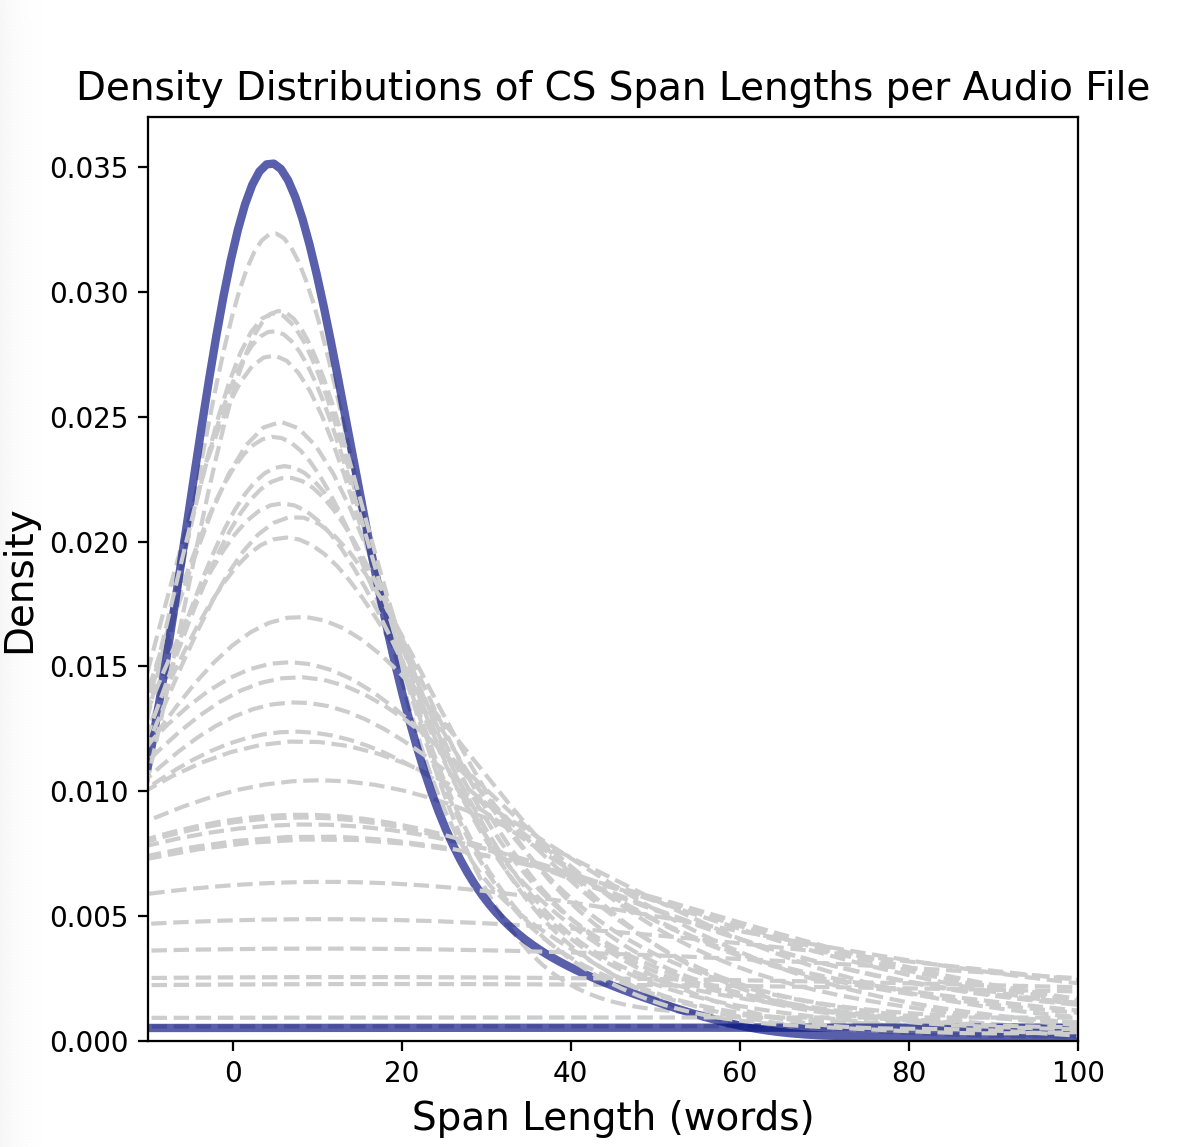
\includegraphics[width=\textwidth]{images/density_spans.png}
    \caption{Span length distributions per transcription.}
    \label{densities}
  \end{subfigure}
  \hfill
  \begin{subfigure}[b]{0.45\textwidth}
    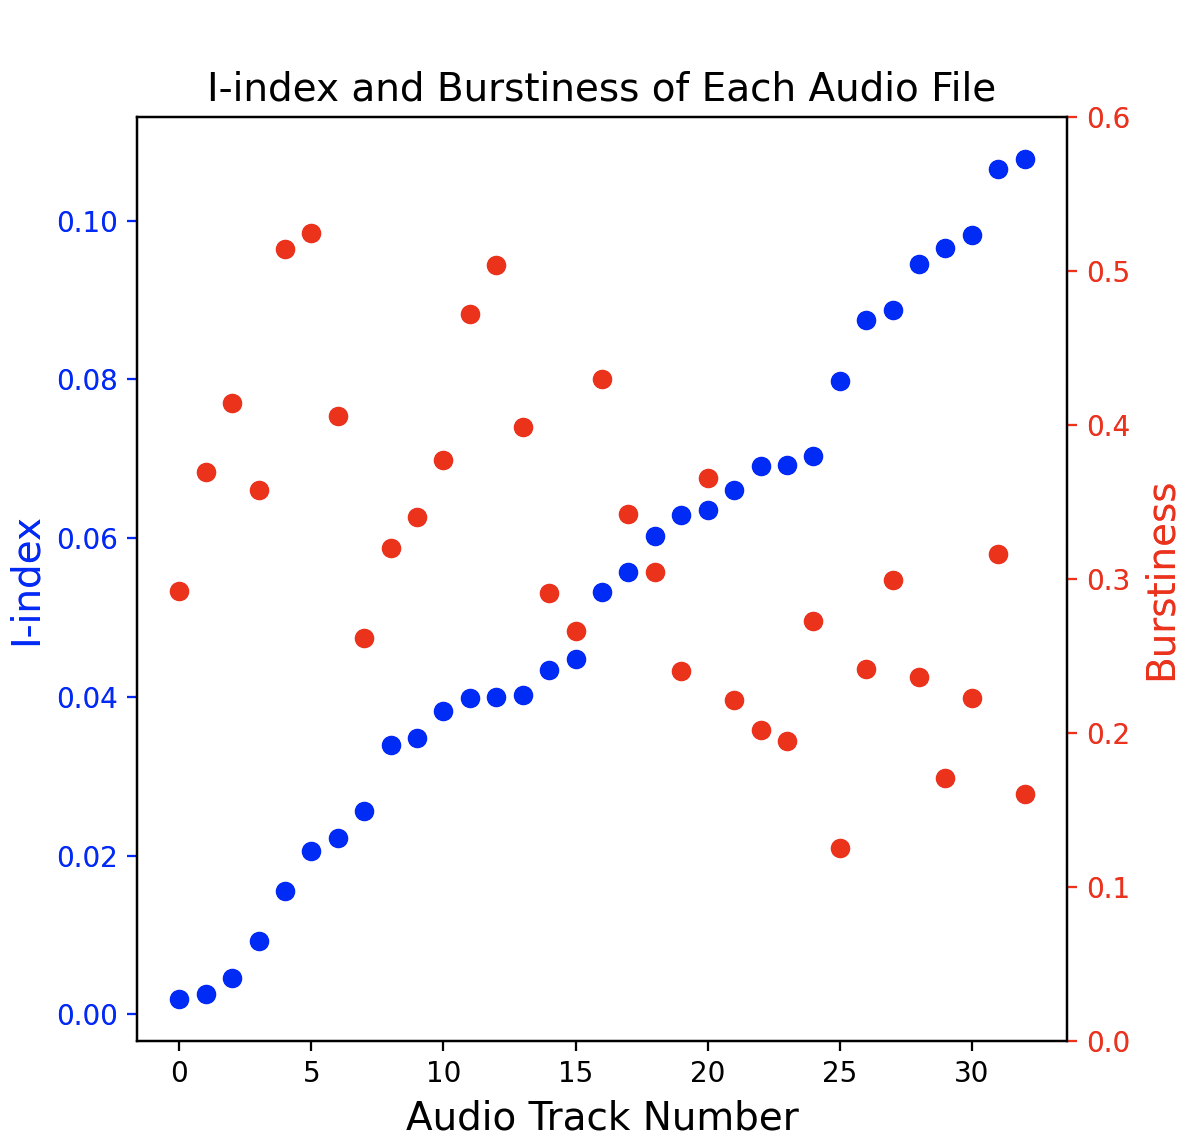
\includegraphics[width=\textwidth]{images/metrics.png}
    \caption{I-index and Burstiness for each audio track.}
    \label{metrics}
  \end{subfigure}
  \caption{Characteristics of the dataset.}
  \label{fig:two_figs}
\end{figure}



% 1. identified what needs to happen to convert chat to rttm 
% 2. createed a workflow to make this conversion, pyannote metrics, python classes/OOP
% 4. ran CS metrics
% 5. Identified which tracks can be modified for the baseline

%Plan (about 1/4 page): Discuss progress in relation to existing project 
%plan and spell out a clear view of what will be done in Thesis/Term C.
\subsection*{Plans}
Building upon the tools developed in thesis B, the conversion of the MIAMI 
corpus into a dataset suitable for SD can now commence. The immediate next 
step is to carry out the manual timestamp corrections required to complete 
the conversion. A 20-minute segment took approximately 1 hour to convert.
Therefore, the conversion of a 16-hour dataset is projected to take around 
50 hours. This work will be undertaken during the term break, prior to 
Thesis C. Once the dataset is ready, the diarization will be performed 
on the monolingual audio tracks to establish a baseline, then applied to 
the CS dataset to understand the impacts of CS on diarization.

\vspace*{10pt}
The diarization error rates can then be compared with the i-index and 
burstiness of the tracks to identify potential correlations between 
language switching frequency and error rates. Lastly, a specially developed
tool will be used to examine the precise points of error in the audio to
determine whether errors predominantly occur during a language switch.
The findings and any conclusions will be documented and presented in the final 
poster and report.



\newpage
\section*{Meeting Log}
\bibliographystyle{IEEEtran}
\bibliography{pubs}
\end{document}








%\begin{wrapfigure}{l}{0.5\textwidth}
%  \centering
%  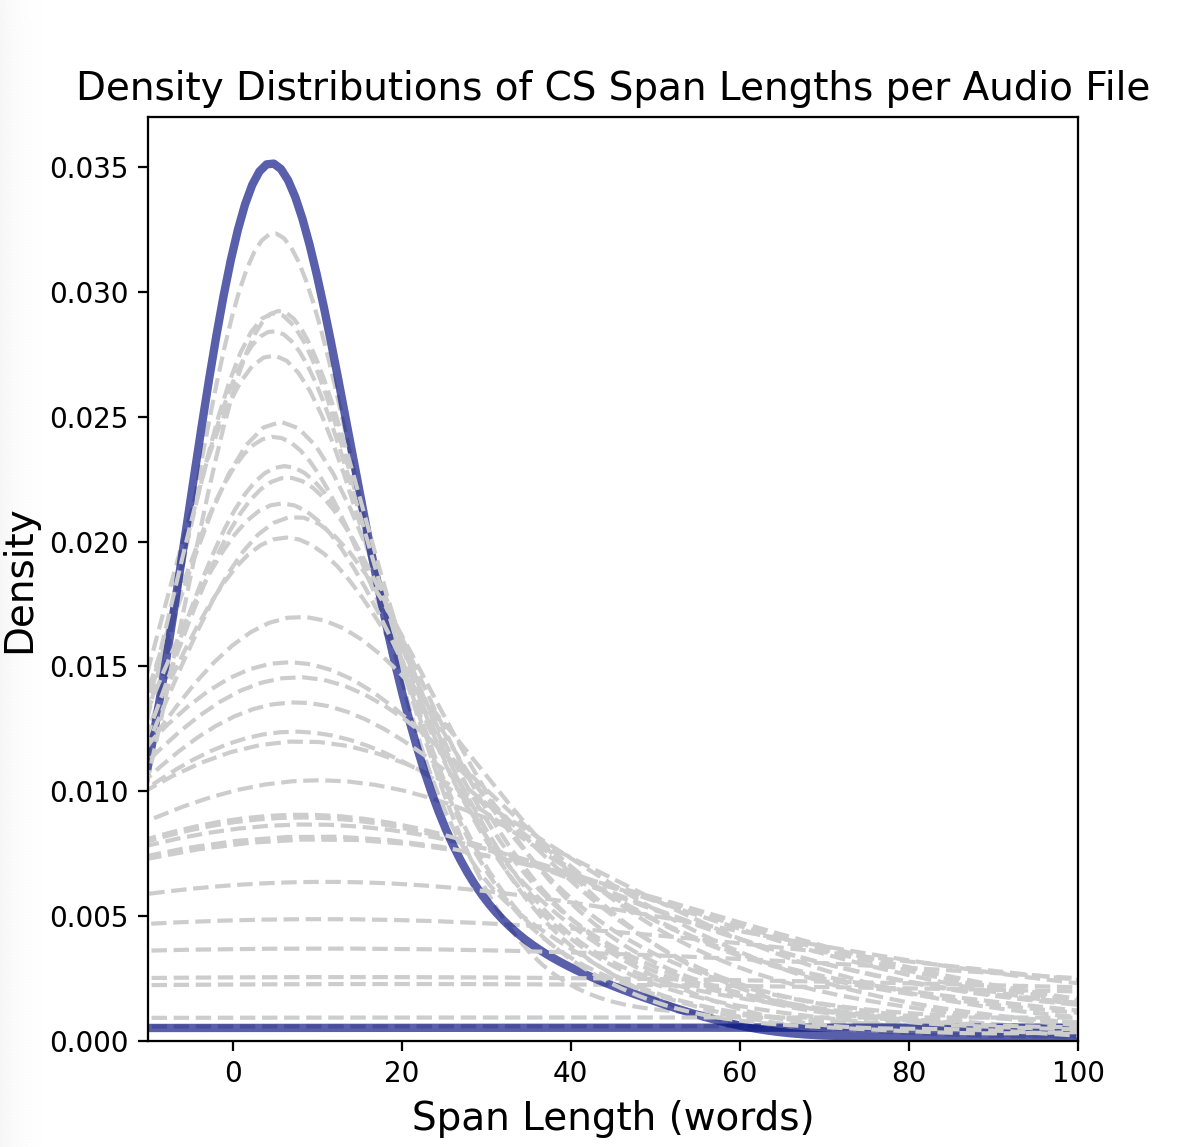
\includegraphics[width=0.5\textwidth]{images/density_spans.png}
%  \caption{A caption for the figure}
%\end{wrapfigure}

